\PassOptionsToClass{12pt}{revtex4-1}
\documentclass[apj]{emulateapj}

\usepackage{tikz}
\usepackage{subfigure}
\usetikzlibrary{shapes.geometric, arrows}
\tikzset{
  int/.style={circle, draw=black, fill=green!20, minimum size=3em},
  int1/.style={circle, draw=black, fill=red!20, minimum size=3em},
  int2/.style={circle, draw=black, fill=blue!20, minimum size=3em},
  init/.style={pin distance=1.2cm,pin edge={loop,thin,black}}
}
\tikzstyle{arrow} = [thick,black,->,>=stealth]
\tikzstyle{pinstyleto} = [pin edge={<-,thick,black}]
\tikzstyle{pinstyleout} = [pin edge={->,thick,black}]


\begin{document}


\slugcomment{STAT 841/ CM 763: Statistical Learning - Classification}
\shorttitle{Conversational Entities}
\shortauthors{Dumont, Khan, Selby, \& Zhi}
%%%Title and author name
\title{Constructing Textual Artificial Conversational Entities \\ using Deep Learning}
\author{\sc{\bfseries Group 2:}\\
\small \emph{Nicole Sandra-Yaffa Dumont } \\
 \small \emph{Sakif Hossain Khan } \\
 \small  \emph{Kira Aveline Selby } \\
 \small  \emph{Congcong Zhi } } 
\affil{University of Waterloo}
%%%

%%%Abstract
\begin{abstract}
an abstract goes here

\end{abstract}
%%%

\section{Background}
some background

\section{Methods}
\subsection{\raggedright Recurrent Neutral Networks (RNNs)} 
\indent
an example flow chart
\begin{center}
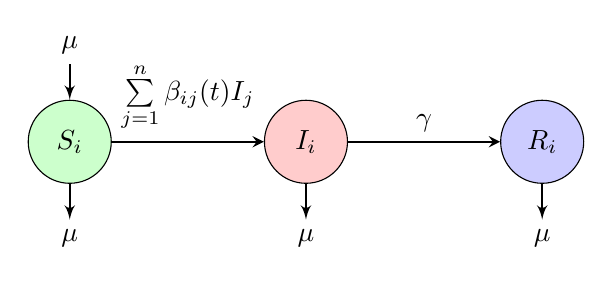
\begin{tikzpicture}[node distance=3cm,auto,>=latex',every node/.append style={align=center}]
    \node [int, pin={[pinstyleto]above:$\mu$}, pin={[pinstyleout]below:$\mu$}] (a)              {$S_i$};
    \node [int1, pin={[pinstyleout]below:$\mu$}] (b) [right of=a] {$I_i$};
    \node [int2, pin={[pinstyleout]below:$\mu$}] (c) [right of=b] {$R_i$};
    
    \draw [arrow] (a) -- node[anchor=south] {$ \sum\limits_{j=1}^{n}\beta_{ij}(t) I_j $} (b);
    \draw [arrow] (b) -- node[anchor=south] {$\gamma$} (c);
\end{tikzpicture}
\end{center}

\subsection{The seq2seq Model} 
\subsubsection{Attention} 
\subsubsection{Beam Search} 


\section{Results}
results go here

\section{Conclusion} 
a conclusion

 

\begin{thebibliography}{99}

\end{thebibliography}

\end{document}